\documentclass[aspectratio=169]{beamer}
\usepackage[utf8]{inputenc}
\usepackage{hyperref}
\usepackage{amsmath,amsfonts,amsthm,bm}
\usepackage{color}
\usepackage{graphicx} % Allows including images
\usepackage{subcaption}
\usepackage{booktabs} % Allows the use of \toprule, \midrule and \bottomrule in tables
\usepackage{tikz}
%\usepackage{pgfplots}
\usepackage{listings}
\usepackage{courier}
\usepackage[version=4]{mhchem}
\usepackage{array}

\lstset{ %
  basicstyle=\scriptsize\ttfamily, % fonts that are used for the code
  breakatwhitespace=false,         % sets if automatic breaks should only happen at whitespace
  %breaklines=true,                 % sets automatic line breaking
  %captionpos=b,                    % sets the caption-position to bottom
  commentstyle=\color{gray}\textit,    % comment style
  keepspaces=true,                 % keeps spaces in text, useful for keeping indentation of code (possibly needs columns=flexible)
  keywordstyle=\color{blue},       % keyword style
  language=Python,                 % the language of the code
  %otherkeywords={*,...},          % if you want to add more keywords to the set
  rulecolor=\color{black},         % if not set, the frame-color may be changed on line-breaks within not-black text (e.g. comments (green here))
  showspaces=false,                % show spaces everywhere adding particular underscores; it overrides 'showstringspaces'
  showstringspaces=false,          % underline spaces within strings only
  showtabs=false,                  % show tabs within strings adding particular underscores
  stringstyle=\color{red}, % string literal style
  tabsize=4,	                   % sets default tabsize to 2 spaces
  columns=fixed                    % Using fixed column width (for e.g. nice alignment)
}

\hypersetup{
    colorlinks=true,
    linkcolor=red,
    filecolor=magenta,      
    urlcolor=red,
}

\DeclareMathOperator*{\argmax}{argmax}
\DeclareMathOperator*{\argmin}{argmin}
\let \vec \mathbf

\newcommand{\classname}{NANO266}
\newcommand{\classyear}{Fall 2024}
\mode<presentation> {
    \usetheme{CambridgeUS}
    \setbeamertemplate{footline}[text line]{%
      \parbox{\linewidth}{\vspace*{-8pt}\classname\hfill\classyear\hfill\insertpagenumber}}

    %\setbeamertemplate{footline}[page number]
    \setbeamertemplate{navigation symbols}{}
}


\title[\classname Lab 1]{\classname~- Quantum Mechanical Modeling of Materials and Nanostructures\\Lab 1}

\author{Shyue Ping Ong}
\institute[UCSD]{University of California, San Diego\\
\medskip
}
\date{\classyear} % Date, can be changed to a custom date

\begin{document}


\begin{frame}
    \titlepage % Print the title page as the first slide
\end{frame}


\begin{frame}{Haber-Bosch Process}
    \centering{\huge{\ce{N_2 + H_2 \rightarrow NH3}}}
    \begin{figure}
        \centering
        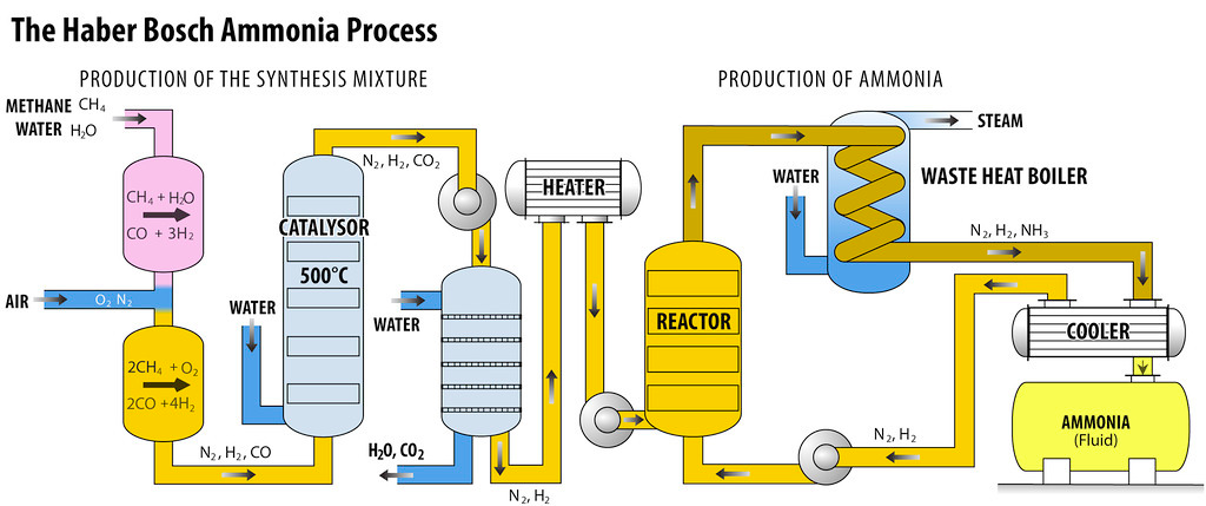
\includegraphics[width=0.8\linewidth]{lectures/figures/Lab1_Haber_Bosch.png}
    \end{figure}
    
\end{frame}


\begin{frame}{One of the most important processes to mankind...}
\begin{figure}
    \centering
    \begin{subfigure}{0.25\textwidth}
    
\includegraphics[width=\linewidth]{lectures/figures/Lab1_Alchemy_of_Air.png}
    \end{subfigure}
    \begin{subfigure}{0.4\textwidth}
    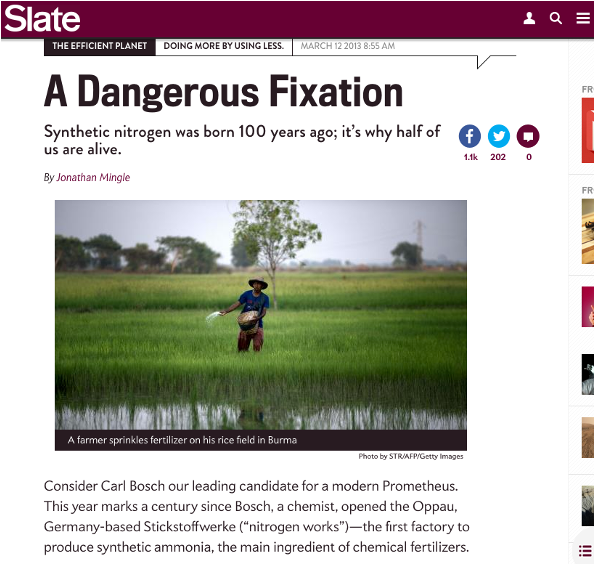
\includegraphics[width=\linewidth]{lectures/figures/Lab1_Dangerous_Fixation.png}
    \end{subfigure}
\end{figure}
\end{frame}

\begin{frame}{Nwchem}
Provide its users with computational chemistry tools that are scalable both in their ability to treat large scientific computational chemistry problems efficiently, and in their use of available parallel computing resources from high-performance parallel supercomputers to conventional workstation clusters. \newline
\newline
Actively developed and maintained by the EMSL at PNNL.\newline
\newline
Distributed as open-source under Educational Community License version 2.0 (ECL 2.0).\newline
\newline
\url{http://www.nwchem-sw.org/}

\end{frame} 

\begin{frame}{Getting started}
\begin{enumerate}
    \item Follow instructions at \url{https://github.com/materialsvirtuallab/nano266/tree/master/labs}
    \item Login to Expanse.
    \item Clone the nano266 github repo with the following command:

       git clone https://github.com/materialsvirtuallab/nano266.git 

    \item Go into the lab1 directory

       cd nano266/labs/lab1

    \item Start simulating!

\end{enumerate}
\end{frame} 


% \begin{frame}[allowframebreaks]{Bibliography}
%     \bibliographystyle{unsrt}
%     \bibliography{refs}
% \end{frame}



\begin{frame}
    \Huge{\centerline{The End}}
\end{frame}

\end{document}

